%\documentclass[a4paper]{article}
\documentclass[10pt,a4paper]{article}
\usepackage[utf8x]{inputenc} % para poder usar tildes en archivos UTF-8
\usepackage[spanish,es-tabla]{babel}
\usepackage{verbatim}
\usepackage{clrscode3e}
\usepackage{amssymb}
\usepackage{graphicx}
\usepackage{float}
\usepackage{pdfpages}

%\usepackage{bibtex}

%\usepackage{a4wide} % márgenes un poco más anchos que lo usual

\usepackage{caratula} % Se puede descargar en ~> https://github.com/bcardiff/dc-tex
\usepackage[breaklinks=true]{hyperref}


\begin{document} % Todo lo que escribamos a partir de aca va a aparecer en el documento.

%fran
%\sloppy

% Completar los datos de la caratula
\titulo{Trabajo Práctico 3 - Tomografía computada} 
\fecha{\today}
\materia{Métodos Numéricos}
\grupo{Grupo "Greco-Herrera-Kubrak-Salvador"}

% Completar los integrantes del grupo:)
\integrante{Cristian, Kubrak}{456/15}{Kubrakcristian@gmail.com}
\integrante{Marcela Alejandra, Herrera}{1162/84}{marcelaalejandraherrera@yahoo.com.ar}
\integrante{Luis Fernando, Greco}{150/15}{luifergreco@gmail.com}
\integrante{Alejo, Salvador}{467/15}{alejo.antonio.salvador@gmail.com}


\maketitle
\par \textbf{Abstract:} El objetivo del Trabajo es realizar la simulación de una tomografía computada partiendo de imágenes tomográficas reales en formato 16 bits. La simulación se realiza generando una simulación de rayos X que atraviesan la imagen, la cual es discretizada en una cuadrícula de tamaño parametrizable. Una vez generados los rayos se realiza la reconstrucción de la imagen utiizando el método de cuadrados mínimos lineales, se realiza una evaluación de resutados usando error cuadrático medio y la reconstrucción de la imagen en formato pgm de 8 bits.

\par  \textbf{Palabras clave:} reconstrucción de imagen tomográfica - cuadrados mínimos lineales - error cuadrático medio
% Aca comienzan a escribir su informe
\tableofcontents


\newpage

\section{Introducción}
\subsubsection*{Introducción}
\par El objetivo del trabajo práctico es evaluar un método para reconstruir imágenes tomográficas sujetas a ruido, utilizando el método de aproximación por cuadrados mínimos.

\par En la toma de una tomografía se emiten rayos X que atraviesan al sujeto en estudio y se realizan múltiples mediciones sobre los mismos para compensar los errores de medición que pudieran producirse. Este proceso conduce a un sistema de ecuaciones lineales sobredeterminado que en general no tiene solución, razón por la cual se utiliza el método de cuadrados mínimos para aproximar una solución.
En nuestro caso para simplificar el problema suponemos que las mediciones que se realizan son de los tiempos que les lleva a los rayos X atravesar el sujeto.

\par Los rayos se emiten de tal forma que atraviesan al sujeto en un plano dado y en distintos ángulos y con diferentes direcciones sobre ese plano.
\par En nuestro caso para simplificar el problema suponemos que las mediciones que se realizan son de los tiempos que les lleva a los rayos X atravesar el sujeto.
\par La superficie del corte a estudiar se discretiza dividiéndola en celdas de acuerdo a una cuadrícula de $n*n$, donde $n$ es un número entero. Cada celda puede ser atravesada por múltiples rayos, de hecho esto es recomendable para poder recolectar una cantidad de datos representativa que permita compensar errores numéricos.
Con los datos recolectados se plantea un sistema de ecuaciones lineales donde los coeficientes están dados por la distancia que recorre cada rayo dentro de cada una de las celdas de la cuadrícula, el vector independiente viene dado por los tiempos que demora de cada rayo en atravesar al sujeto y las incógnitas son las velocidades de los rayos dentro de cada celda. Estas velocidades son una propiedad de la materia atravesada.

\par Para evaluar la calidad de la reconstrucción de la imagen tomográfica utilizamos como métrica el cálculo del Error Cuadrático Medio, el cual va a comparar las velocidades de cada celda obtenidas a partir de las imágenes sin ruido contra las velocidades calculadas por medio de cuadrados mínimos.

\par Utilizamos la técnica de k-fold a la base de imágenes para generamos un conjunto de datos de entrenamiento y otro de datos de testing a fines de elegir los mejores valores para el $n$ de la discretización, el nivel de ruido y la cantidad y distribución de los rayos.

\par Centrándonos en nuestro caso, debido a que no es posible la utilización de un tomógrafo real para recolectar los datos, utilizamos imágenes de una base de datos de imágenes tomográficas (http://www.via.cornelledu/databases/). A partir de estas imágenes generamos las instancias de prueba que se van a convertir en nuestro "sujeto" en estudio tal como se detalla más abajo.

\par Usamos las imágenes de partida como si fuera el sujeto al que necesitamos estudiar y simulamos matemáticamente los rayos X, agregando ruido aleatorio para simular los errores de medición. Decidimos utilizar dos formas de manejar el ruido:
a) modificando la intensidad de los pixeles de la imagen elegida como sujeto, utilizando valores aleatorios con distribución gaussiana, para luego hacer la simulación de los rayos X sobre la imagen ruidosa.
b) Calculando los tiempos de recorrida de cada rayo simulado, a través de la imagen sin ruido, y luego perturbando los valores obtenidos.

\par La granularidad de la discretización, la cantidad y dirección de los rayos y el nivel de ruido utilizado son parámetros de experimentación. En su determinación tenemos en cuenta un compromiso entre la calidad de la imagen reconstruída y los tiempos de ejecución (principalmente en la resolución del sistema por cuadrados mínimos). Para la resolución del sistema utilizamos las ecuaciones normales y en este caso el aumento en la dimensión de la matriz generadas está íntimamente relacionada con el tiempo de procesamiento.

\subsubsection*{nombre}

\newpage

% \section{Demostraciones}
% \newpage

\section{Desarrollo}
\subsubsection*{Desarrollo}

\title {Imágenes}

\par Para realizar la experimentación utilizamos la imagen tomo.png provista por la cátedra, con una resolución de 100 x 100 pixeles.
\par La imagen la trabajamos en formato .csv para la entrada con una profundidad de 16 bits y luego de la reconstrucción la guardamos en formato pgm de 8 bits.
\par Para la conversión de la imagen de 16 a 8 bits implementamos una función (to8bits) que identifica los valores de intensidad máximo y mínimo de la imagen a guardar. Al valor mínimo se le asocia el valor de salida 0 y al máximo el valor de salida 255. Los valores de intensidades intermedias se distribuyen de forma proporcional. Este procedimiento permite salvar el inconveniente de que como resultado de la eliminación gaussiana se pueden obtener valores negativos, los cuales no tienen sentido en este contexto ya que representan intensidades que siempre son valores mayores o iguales a cero, o valores mayores al máximo valor permitido para una imagen de 16 bits. Esto es posible porque estamos encontrando una solución aproximada y además estamos trabajando con ruido.

\par En un principio comenzamos utilizando los archivos .csv provistos por la cátedra de 512 x 512 pixeles, con estas imágenes realizamos varias pruebas fallidas que se explican más detalladamente en el apartado Generación de rayos. Debido a diversas dificultades que se nos presentaron con la elección de la estrategia para trazar los rayos, se demoró el inicio de las pruebas y optamos por utilizar imágenes más chicas para poder realizarlas en el tiempo de que disponíamos. Aunque hubiera sido interesante poder trabajar con un conjunto mayor de imágenes.

\title {Discretización} Para discretizar la imagen utilizamos valores divisores de 100. En los tests de granularidad, variamos el tamaño de las celdas tomando los valores 4x4, 5x5, 10x10, 20x20, 25x25 y 50x50 pixeles. Como ya se analizó a medida que se achica el tamaño de las celdas crece el tiempo de procesamiento, lo cual condicionó la elección de los parámetros.

\title {Cálculo de la distancia recorrida por cada rayo} 
Implementamos una función ''pasa'' que se encarga de identificar por qué pixeles pasa un rayo (los rayos son considerados como rectas en el plano, caracterizados por un punto de origen que llamamos $(x_{0},y_{0})$ y un ángulo $\alpha$ ).

\par Para poder describir esta función adecuadamente imaginamos la imagen ubicada en un eje de coordenadas de modo tal que su vértice inferior izquierdo se encuentre en la coordenada (0,0). Pensamos a la imagen como un subconjunto de puntos del plano.

\par Utilizando la tangente de $\alpha$ (que es la pendiente de la recta asociada al rayo), se busca la intersección con la recta $y=0$ la cual es el punto $(x-y/tangent(\alpha),0)$.  De ahi en mas se utiliza la ecuación de la recta $y=tan(\alpha)*x+y_{0}$, variando el valor de $x$ para calcular los puntos del plano (siempre hablando del plano en un sentido general) por los que pasa la recta. Si el punto hallado pertenece a la imagen se guardan las coordenadas del pixel correspondiente en un vector, para ser usadas posteriormente para el cálculo de distancias y de tiempos.

\par Esta función se usa para calcular el tiempo que le toma a un rayo atravesar al sujerto. Para esp se hace la suma de las intensidades de los pixeles por las que pasa el rayo ya que la intensidad de los mismos la asociamos al tiempo que le toma a un rayo atravesar el mismo.

\par Finalmente se la reutilizará por ultima vez para calcular la cantidad de pixeles en cada celda por las que pasa el rayo. Para hacer esto se calcula para cada pixel por los que pasa el rayo a qué celda pertenece. Para esto es necesario realizar una conversión en las coordenadas, ya que las celdas de la imagen se identifican desde la esquina superior izquierda.

\par Debido a que los rayos pasan solamente por algunas celdas del total (Se puede ver gráficamente que si la grilla es de n celdas, a lo sumo serán $2*n-1$), para la matriz de distancias reutilizamos la estructura de matriz esparza del TP1.

\title{Generación de rayos}

\par Una de las decisiones que tuvimos que tomar fue de qué forma trazar los rayos simulados que íbamos a aplicar a la imagen.

\par En cuanto a la cantidad de rayos, la misma debe ser mayor que $n^{2}$, siendo $n$ la cantidad de celdas de la discretización, ya que con una cantidad menor habría celdas que no son atravesadas por ningún rayo. En ese caso, hay columnas completas de ceros en la matriz de distancias, lo cual se traduce en filas de ceros en la matriz del sistema a resolver que como ya explicamos en la introducción se obtiene como $D^{t}D t = D^{t} v$. Esta situación se corresponde con un sistema con infinitas soluciones.

\par En cuanto a la ubicación de los emisores, inicialmente pensamos en dos opciones que resultaron fallidas:
\begin{enumerate}
\item Trazar rayos horizontales y verticales, formando una cuadrícula.
\item Trazar rayos saliendo de los cuatro vértices de la imagen en distintos direcciones para barrer los $90^{\circ}$ de cada ángulo.
\end{enumerate}

\par En ambos casos, al comenzar la experimentación nos encontramos con dificultades.

\par En el primer caso al realizar la eliminación gaussiana nos encontrábamos con que la matriz tenía filas completas en cero (matriz no inversible).

\par En el segundo caso, si bien se ejecutaban todos los pasos del programa las imágenes reconstruídas no eran reconocibles.

Al realizar un análisis de estos resultados nos dimos cuenta que los rayos trazados de estas formas eran muy similares entre sí y en consecuencia no suministraban información sufuciente para realizar una buena aproximación a la verdadera solución del sistema. Igualmente adjuntamos la implementación en el código a título informativo.

\par Finalmente decidimos trazar rayos desde los cuatro laterales de la imagen. Los emisores se ubican en igual cantidad sobre los lados de la imagen, la ubicación de los emisores se selecciona aleatoriamente en base a una distribución uniforme entre $0$ y $k$, siendo $k$ la cantidad de pixeles por lado de la imagen (es decir suponiendo que la imagen tiene $k*k$ pixeles).

\par De cada uno de estos emisores salen igual cantidad de rayos en ángulos que van entre $0^{\circ}$ a $180^{\circ}$. Los valores de los ángulos también se seleccionan aleatoriamente con distribución uniforme.

\par Si bien este método es aleatorio -con lo que los resultados difícilmente se repitan en corridas sucesivas- utilizando una cantidad suficientemente grande de rayos (como en este caso) por consecuencia de la Ley de los Grandes Números, en general los rayos quedan bien distribuídos a lo largo (y ancho) de la imagen, pudiendo obtener así resultados consistentes en varias corridas.

\par De los tres métodos este fue el que nos dio mejores resultados y el que terminamos eligiendo para realizar la experimentación.

\par Durante la experimentación, para una discretización de imagen de 10 celdas por lado (100 celdas en total), realizamos dos tipos de pruebas:
\begin{enumerate}
\item Sobre la cantidad de emisores, variando entre 20 y 140, aumentando de a 20 ($2*n$ hasta $7*2*n$). Sin aplicar ruido y manteniendo constante la cantidad de rayos por emisor en 100.
\item Sobre la cantidad de rayos por emisor, variando desde 50 hasta 150, aumentando de a 10.  Sin aplicar ruido y manteniendo constante la cantidad de emisores en 100.
\end{enumerate}

\par En la fig. se puede ver el trazado de rayos resultante tomando como base la imagen tomo.png en un tamaño de 25 x 25 pixeles, con una discretización en celdas de 5 x 5 pixeles, usando 25 emisores y 25 rayos por emisor.

\begin{figure}[H] 
\centering
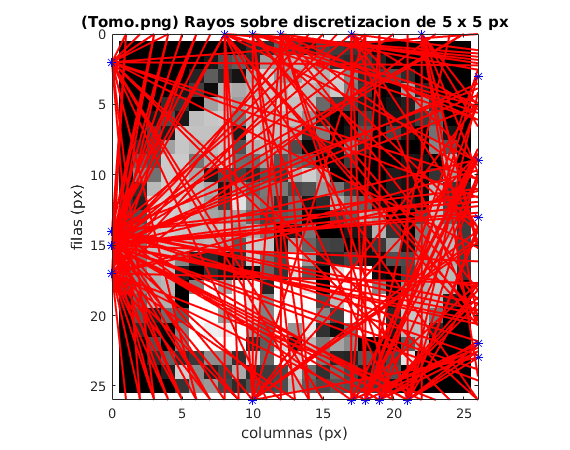
\includegraphics[width=1\textwidth]{img/rayos_tomo25x25px.png}
\caption{Trazado aleatorio de rayos}
\label{fig:rayos aleatorios}
\end{figure}

\title{Cuadrados mínimos} Para resolver el sistema de ecuaciones de cuadrados mínimos utilizamos las ecuaciones normales. Para esto reutilizamos la estructura de matriz esparza y el algoritmo de eliminación gaussiana del TP1, al cual modificamos para utilizar pivoteo de filas.

\par Durante el testeo implementamos la eliminación gaussiana utilizando una matriz completa pero no reportó ningún beneficio en el tiempo de procesamiento por lo cual descartamos la idea.

\title{Ruido} Como explicamos en la introducción utilizamos ruido gaussiano aleatorio multiplicativo sobre el vector de tiempos de recorrida de los rayos de manera que para cada elemento, el resultado luego de aplicar el ruido es $v{1}= v + v * \alpha * x$ con $x$ un valor aleatorio entre 0 y 1 con distribución normal.
Durante la experimentación usamos como parámetro los valores
$x * \alpha$ para $\alpha$ = 0.001 y $x$ tomando valores del conjunto en $\{1,2,3,4,5,6,10,20,50\}$
\par El $\alpha$ actúa como un regulador de ruido. Elegimos que sea multiplicativo (es decir, multiplicando el número aleatorio por el del vector en lugar de por una constante) para que sea consistente la aplicación del ruido. De otra forma, al tener valores en el vector al cuál le vamos a aplicar el ruido que se encuentran comprendidos en un rango muy amplio, si multiplicaramos por una constante estaríamos aplicando proporcionalmente demasiado ruido en algunos valores y muy poco en otros, lo que resultaría en un ruido que deformaría completamente algunas partes de la imagen y dejaría casi intactas otras, cosa que no nos es útil.

\par Otra alternativa que analizamos es aplicar el ruido directamente sobre los pixeles de la imagen, después de calcular los vectores de tiempos de recorrida y de velocidades exactos. Pero finalmente nos decidimos por la utilización del ruido sobre el vector de tiempos. 

%\begin{figure}[H] 
%\centering
%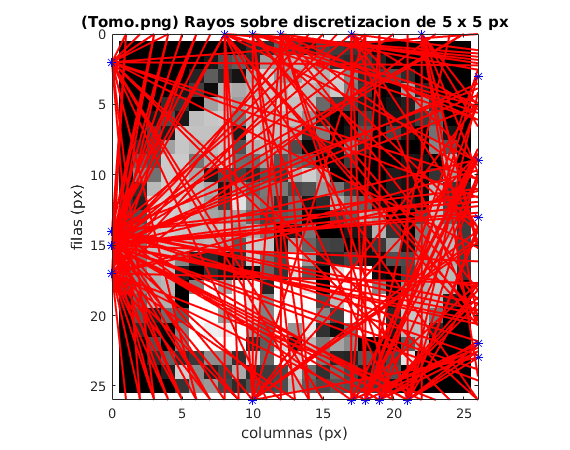
\includegraphics[width=1\textwidth]{img/rayos_tomo25x25px.png}
%\caption{Trazado aleatorio de rayos}
%\label{fig:rayos aleatorios}
%\end{figure}




\newpage

% \section{Experimentación}
% \subsubsection*{Experimentación}
Para experimentar analizamos la influencia en los resultados de las diferentes variables de experimentación que manejamos utilizando tanto el método KNN como el KNN + PCA. 
Las mismas son la cantidad de vecinos considerados por KNN (k), y la cantidad de componentes principales de la imagen transformada ($\alpha$).
Lo hicimos sobre dos bases de datos: una con im\'agenes de tamaño reducido, y otra con imágenes sin reducir (a las cuales llamaremos \textit{big tempo})
Nuestras expectativas previas a la experimentación fueron las siguientes\\
Por un lado consideramos que el tamaño de las im\'agenes influir\'a en el tiempo requerido para su procesamiento pero debido a la mayor informaci\'on disponible,
funciar\'an mejores los algoritmos.\\
Con respecto a la variaci\'on del $k$ en $KNN$ suponemos que con un $k$ ni muy grande ni muy chico, obtendremos buenos resulatados de reconocimiento.\\
Frente a los diferentes algoritmos (KNN o PCA + KNN) creemos que la segunda opci\'on realizar\'a un mejor trabajo pero en un mayor tiempo, por lo que habr\'a que evaluar si se justifica su utilizanci\'on.\\
Por \'ultimo, respecto al par\'ametro $\alpha$ (cantidad de iteraciones del m\'etodo de las potencias) resulta obvio estimar que a mayor $\alpha$, mayor ser\'a el tiempo de ejecuc\'on aunque esperamos que esto
mejore significativamente la tasa de reconocimiento.




% Conclusión:
% Luego de observar estos gráficos llegamos a algunas conclusiones.
% En cuanto al tiempo, por un lado, la cantidad de vecinos cercanos que tomemos no afecta significativamente el tiempo, pero lo que sí lo afecta es el $\alpha$ de PCA.
% A qué se debe esto? Teniendo en cuenta el funcionamiento de nuestro algoritmo, entendemos que esto se debe a que una gran parte del tiempo de procesamiento de PCA se consume en el método de la potencia (que se realiza $\alpha$ veces) y en la transformación de los autovectores calculados en los de la verdadera matriz de covarianza de la muestra, que involucran numerosos cálculos matriciales.

% Sin embargo, pensamos que en una implementación real estaríamos trabajando con una única training base, y las transformaciones que llevamos a cabo en el PCA las haríamos una única vez, con lo que este costo de tiempo se pagaría solamente una vez o cuando sea necesario agregar o quitar alguna imagen, para luego realizar únicamente el reconocimiento. Usando PCA + KNN tenemos la ventaja de trabajar con imágenes de menor tamaño con el consiguiente ahorro de espacio.
% \newpage

\section{Resultados y discusion}
\subsubsection*{Resultados obtenidos}

% \begin{figure}[H]
% 	\centering	\includegraphics[width=0.8\textwidth]{img/nombre.png}
% 	\caption{Titulo}
% 	\label{fig:etiqueta}
% \end{figure}


\begin{figure}[H]
	\centering	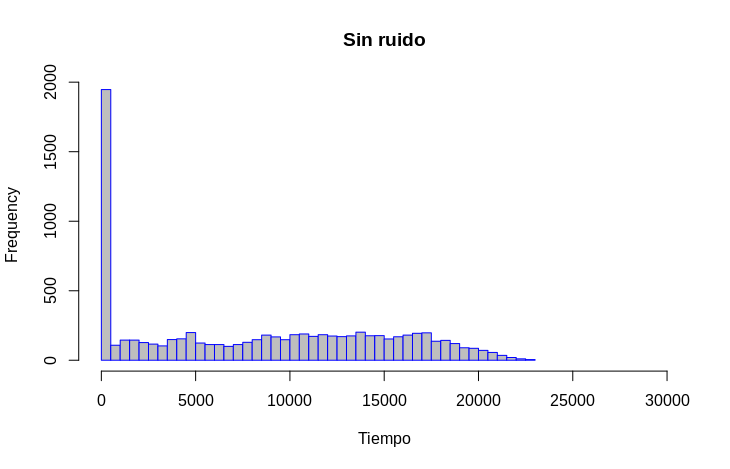
\includegraphics[width=0.7\textwidth]{img/sinRuido.png}
	\caption{Vector de tiempos de rayos sin ruido}
	\label{fig:etiqueta}
\end{figure}
\par Acá podemos observar que efectivamente, el ruido aditivo modifíca mucho más algunas partes del vector mientras que otras no se aprecian muchos cambios. En este caso el histograma de ruido aditivo sufre cambios notorios respecto del vector sin ruido, mientras que en los valores más grandes casi que no notamos se notan diferencias.

\begin{figure}[H]
	\centering	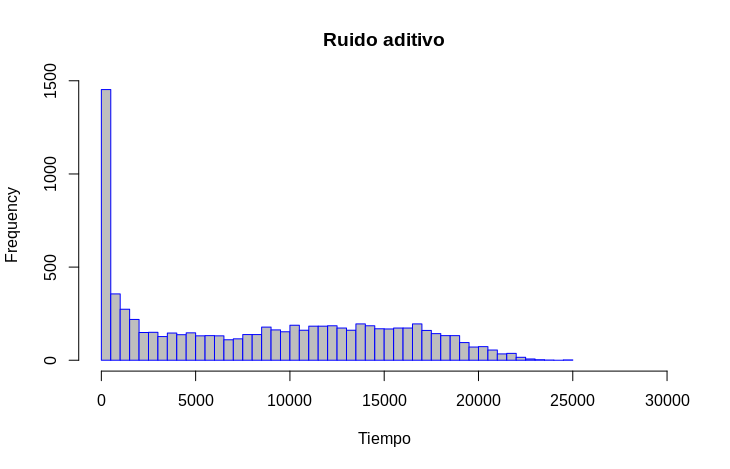
\includegraphics[width=0.7\textwidth]{img/ruidoAditivo.png}
	\caption{Vector de tiempos de rayos con ruido aditivo}
	\label{fig:etiqueta}
\end{figure}

\par En este otro caso en cambio, vemos que las diferencias entre el histograma de ruido multiplicativo y sin ruido existen pero están más uniformemente distribuídas. La única anormalidad que observamos es un incremento en los valores máximos, no obstante se trata de unos pocos casos aislados.
Esto se parece más a lo que esperabamos que hiciera nuestro ruido, por eso fue que elegimos usar este método en nuestra implementación.
\begin{figure}[H]
	\centering	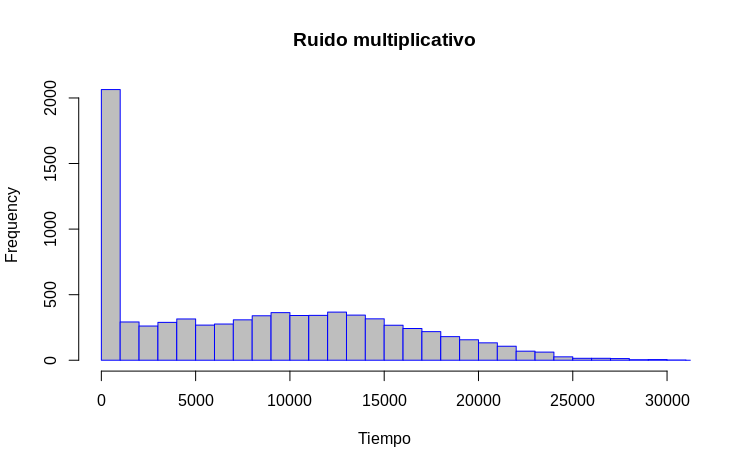
\includegraphics[width=0.7\textwidth]{img/ruidoMultiplicativo.png}
	\caption{Vector de tiempos de rayos con ruido multiplicativo}
	\label{fig:etiqueta}
\end{figure}



\begin{figure}[H]
	\centering	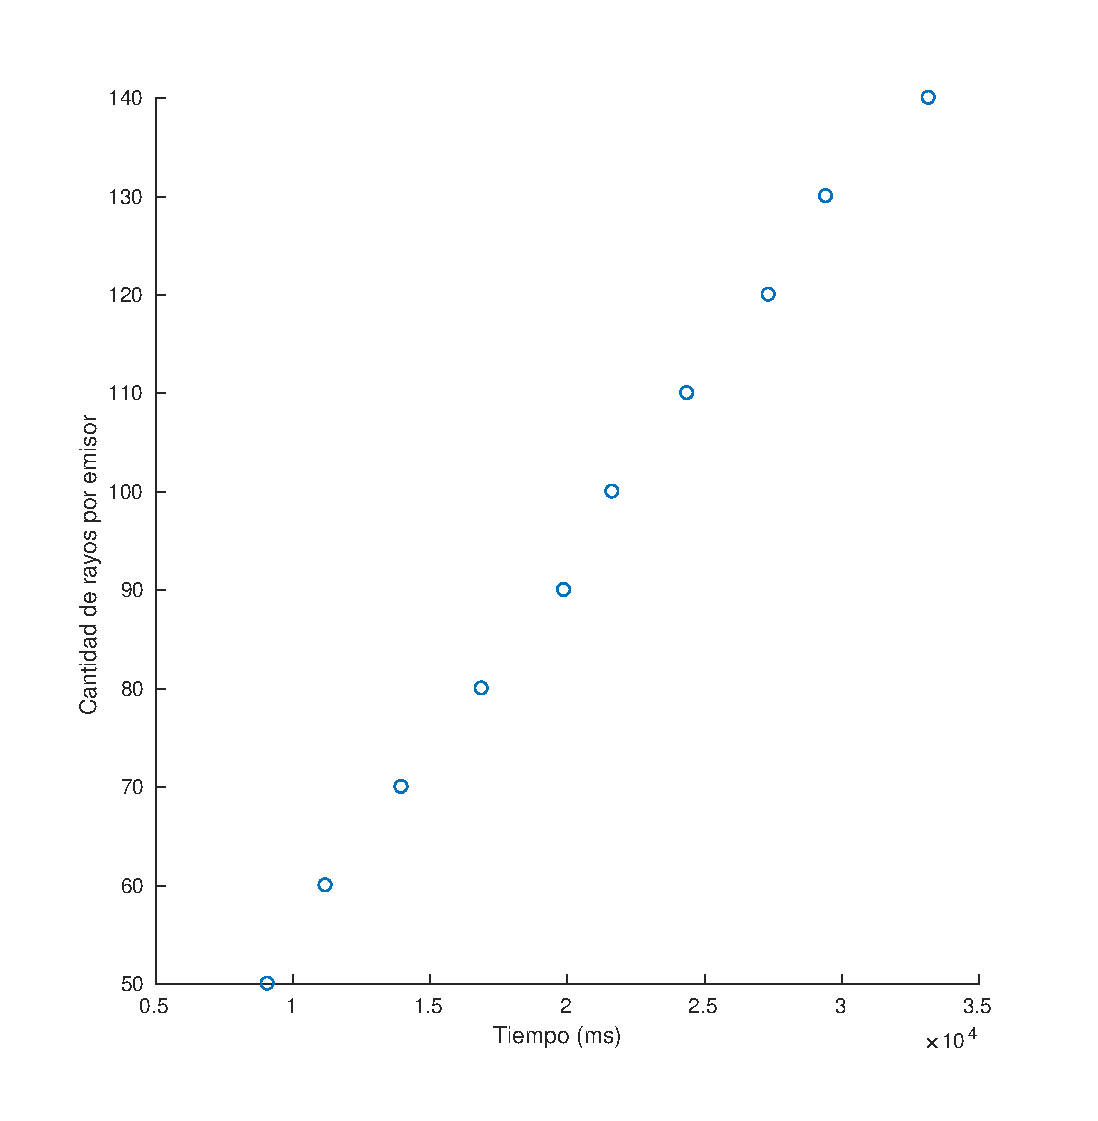
\includegraphics[width=0.7\textwidth]{img/cantrayos_tiempo}
	\caption{Tiempo en funcion de la Cantidad de rayos con granularidad, cantidad de emisores y ruido fijos}
	\label{fig:cantrayos_tiempo}
\end{figure}
\par Tal como se puede apreciar en esta imagen la cantidad de rayos que parten de cada emisor afectan de manera importante el tiempo de ejecuci\'on.


\begin{figure}[H]
	\centering	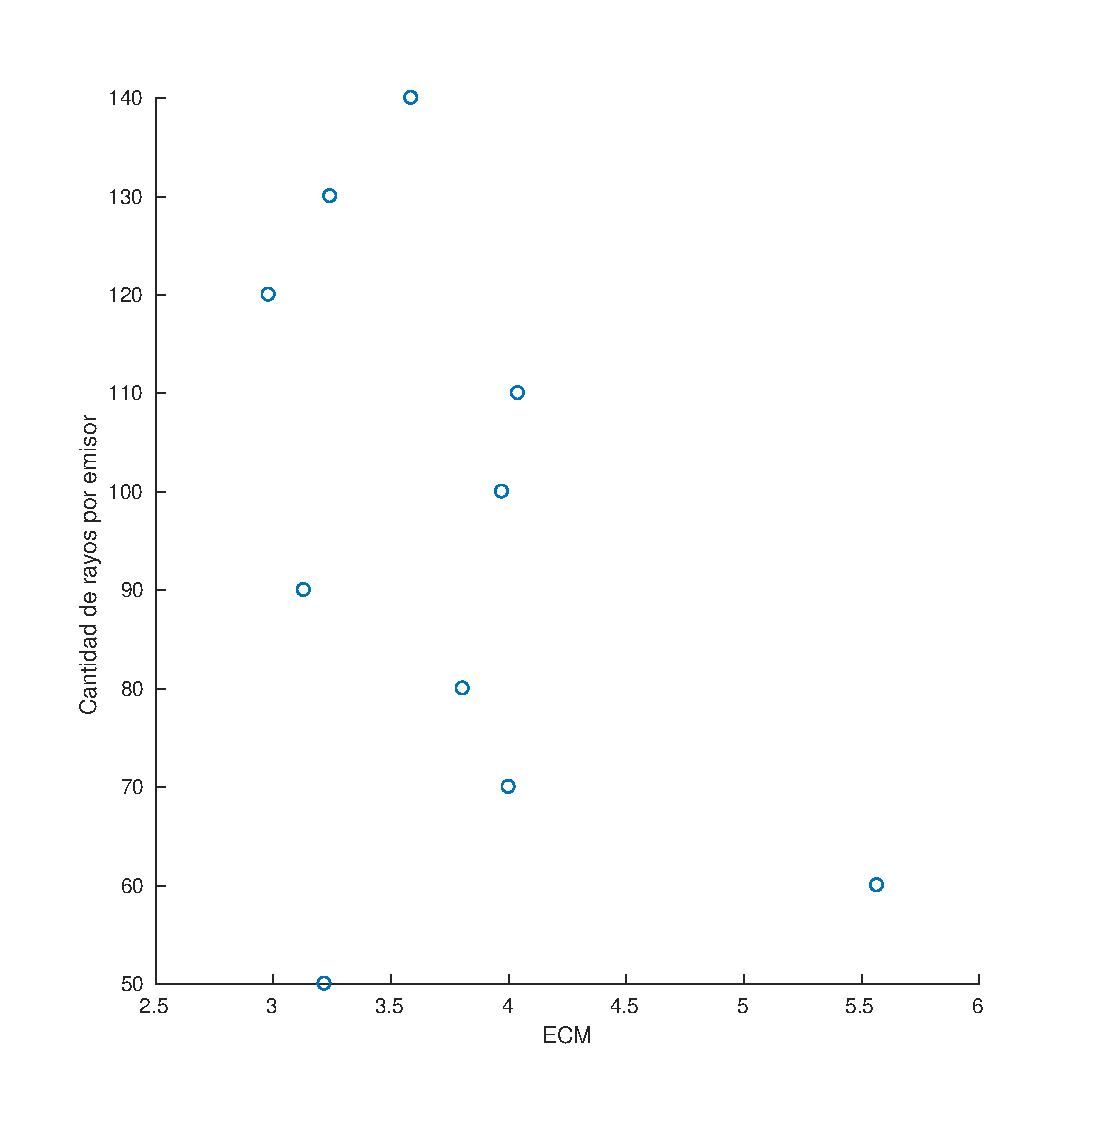
\includegraphics[width=0.7\textwidth]{img/cantrayos_ecm}
	\caption{ECM en funcion de la Cantidad de rayos con granularidad, cantidad de emisores y ruido fijos}
	\label{fig:cantrayos_eps}
\end{figure}


\begin{figure}[H]
	\centering	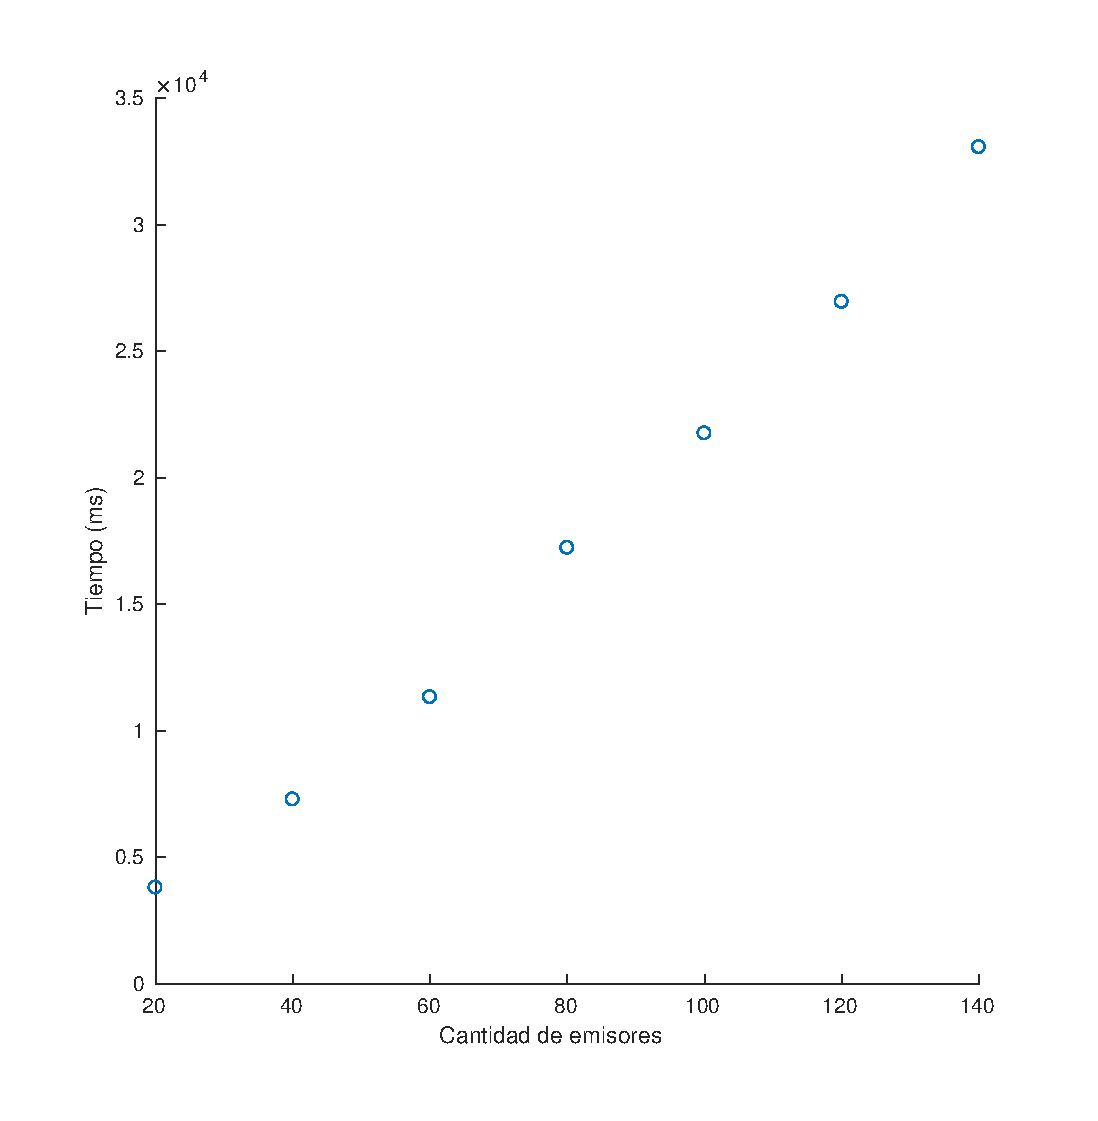
\includegraphics[width=0.7\textwidth]{img/emi_tiempo}
	\caption{Tiempo en funcion de la Cantidad de emisores con granularidad, cantidad de rayos por emisor y ruido fijos}
	\label{fig:emi_tiempo}
\end{figure}
\par Tal como se puede observar en este gr\'afico la cantidad de emisores de rayos afecta de manera directa en el tiempo de ejecuci\'on.

\begin{figure}[H]
	\centering	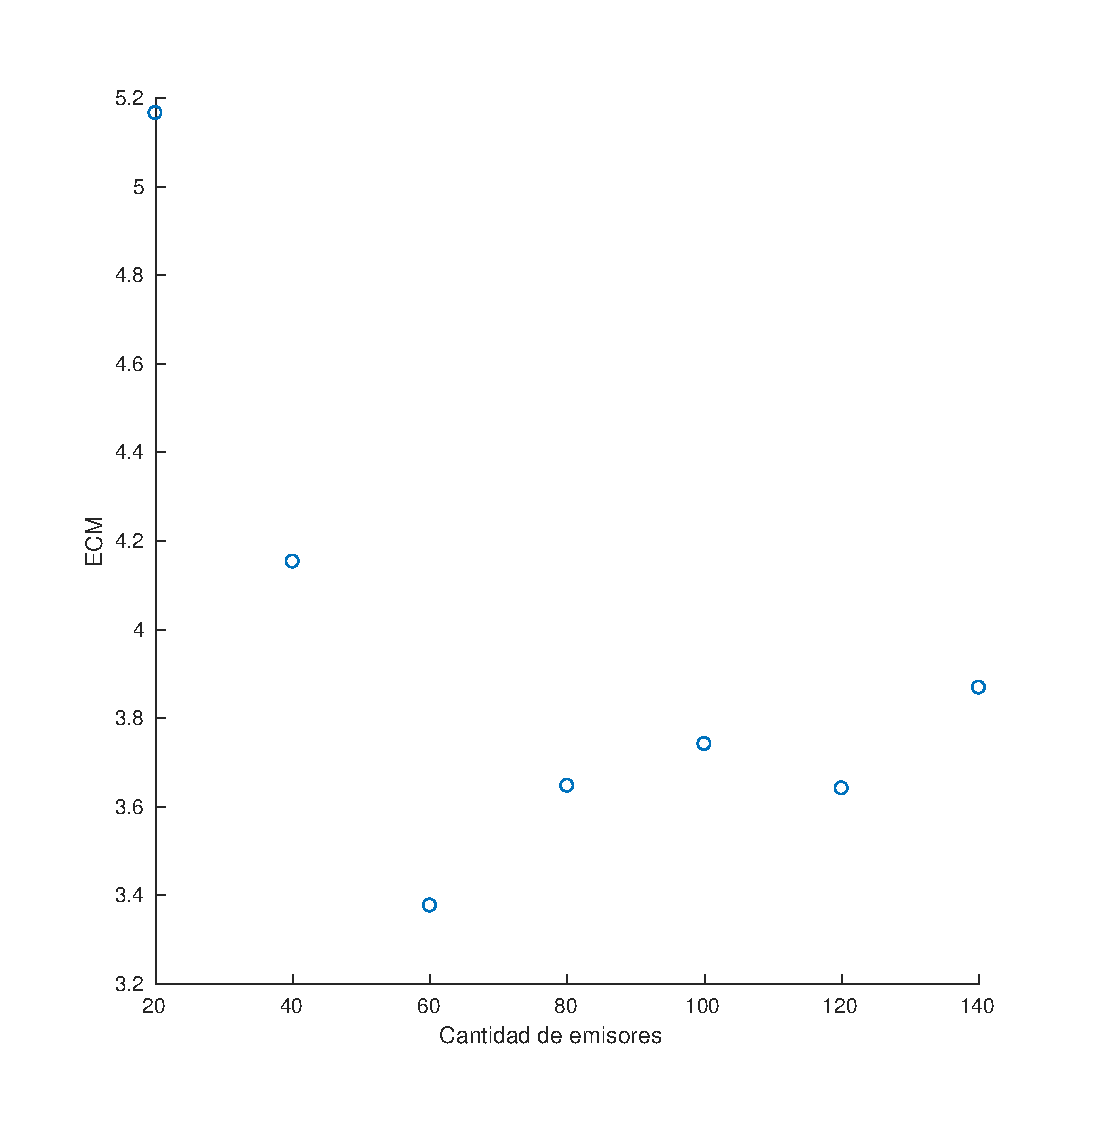
\includegraphics[width=0.7\textwidth]{img/emi_ecm}
	\caption{ECM en funcion de la Cantidad de emisores con granularidad, cantidad de rayos por emisor y ruido fijos}
	\label{fig:emi_ecm}
\end{figure}


\begin{figure}[H]
	\centering	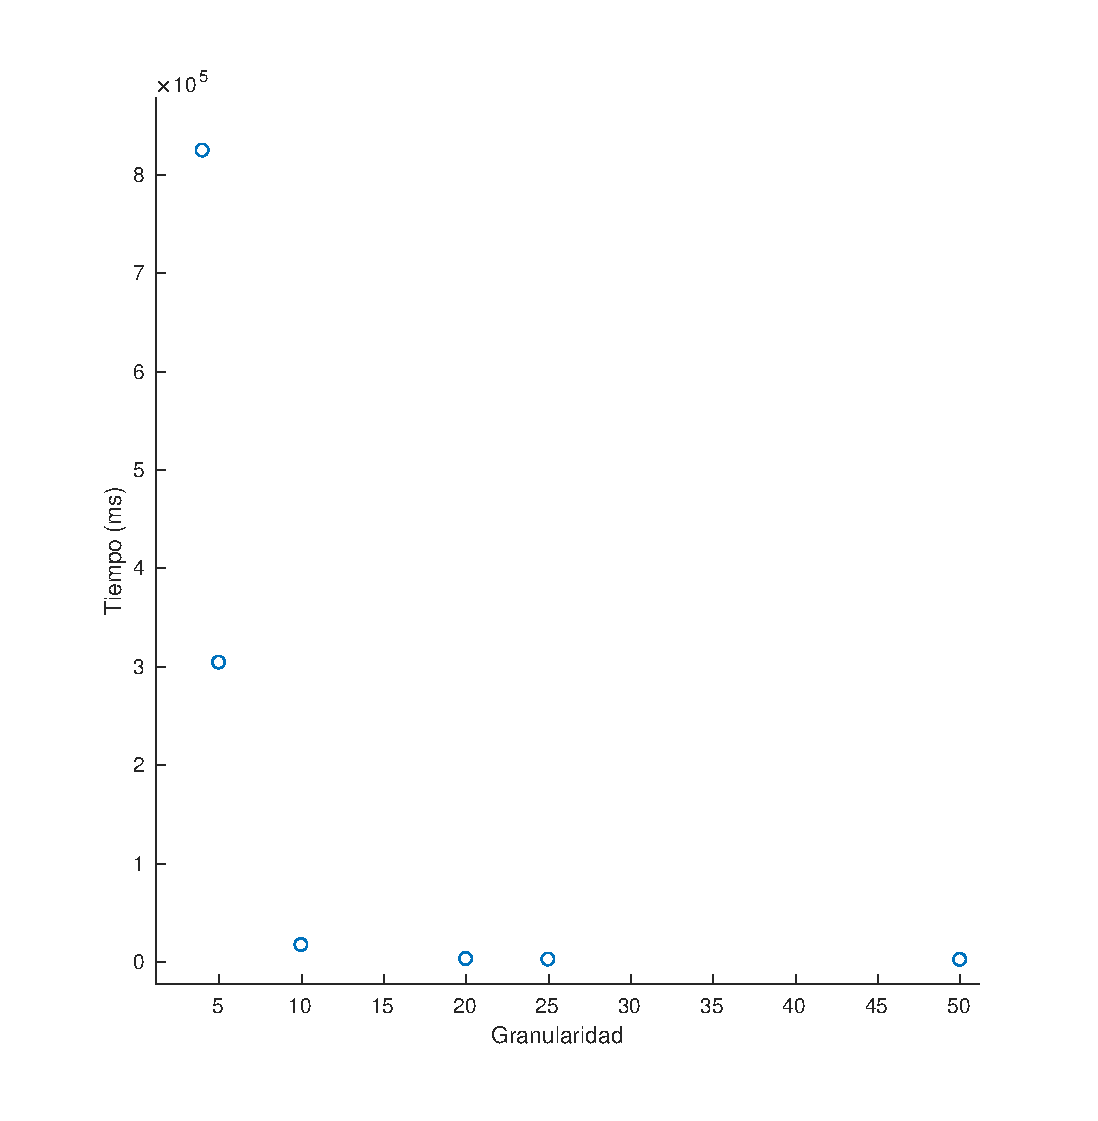
\includegraphics[width=0.7\textwidth]{img/granu_tiempo}
	\caption{Tiempo en funcion de la Granularidad con cantidad de rayos, cantidad de emisores y ruido fijos}
	\label{fig:granu_tiempo}
\end{figure}
\par A mayor granularidad, menor resulta el tiempo de ejecuci\'on debido a que casos de granularidad se reduce el tamaño de la matriz imagen.

\begin{figure}[H]
	\centering	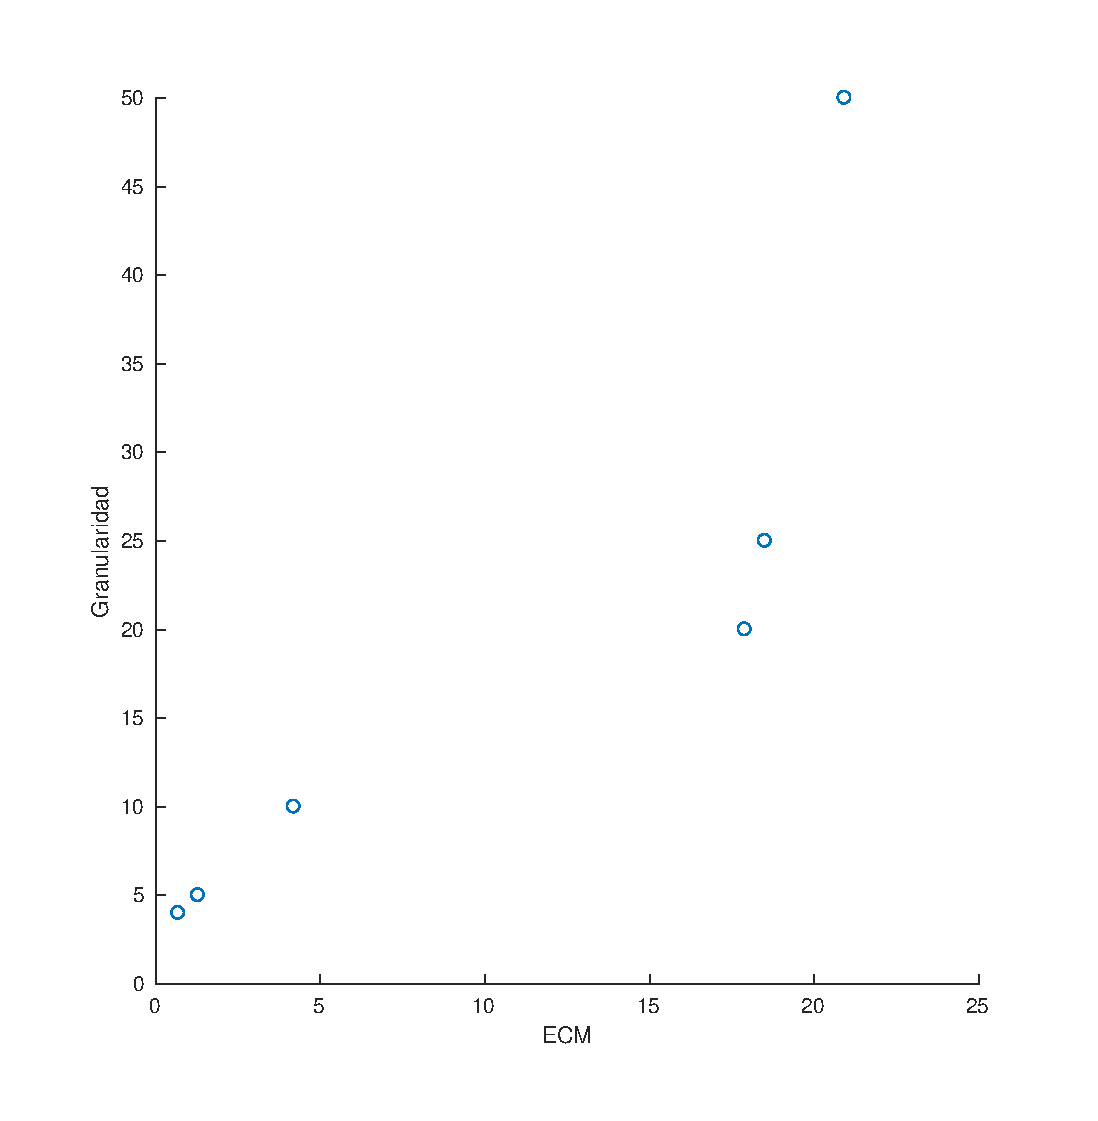
\includegraphics[width=0.7\textwidth]{img/granu_ecm}
	\caption{ECM en funcion de la Granularidad con cantidad de rayos, cantidad de emisores y ruido fijos}
	\label{fig:granu_ecm}
\end{figure}

\begin{figure}[H]
	\centering	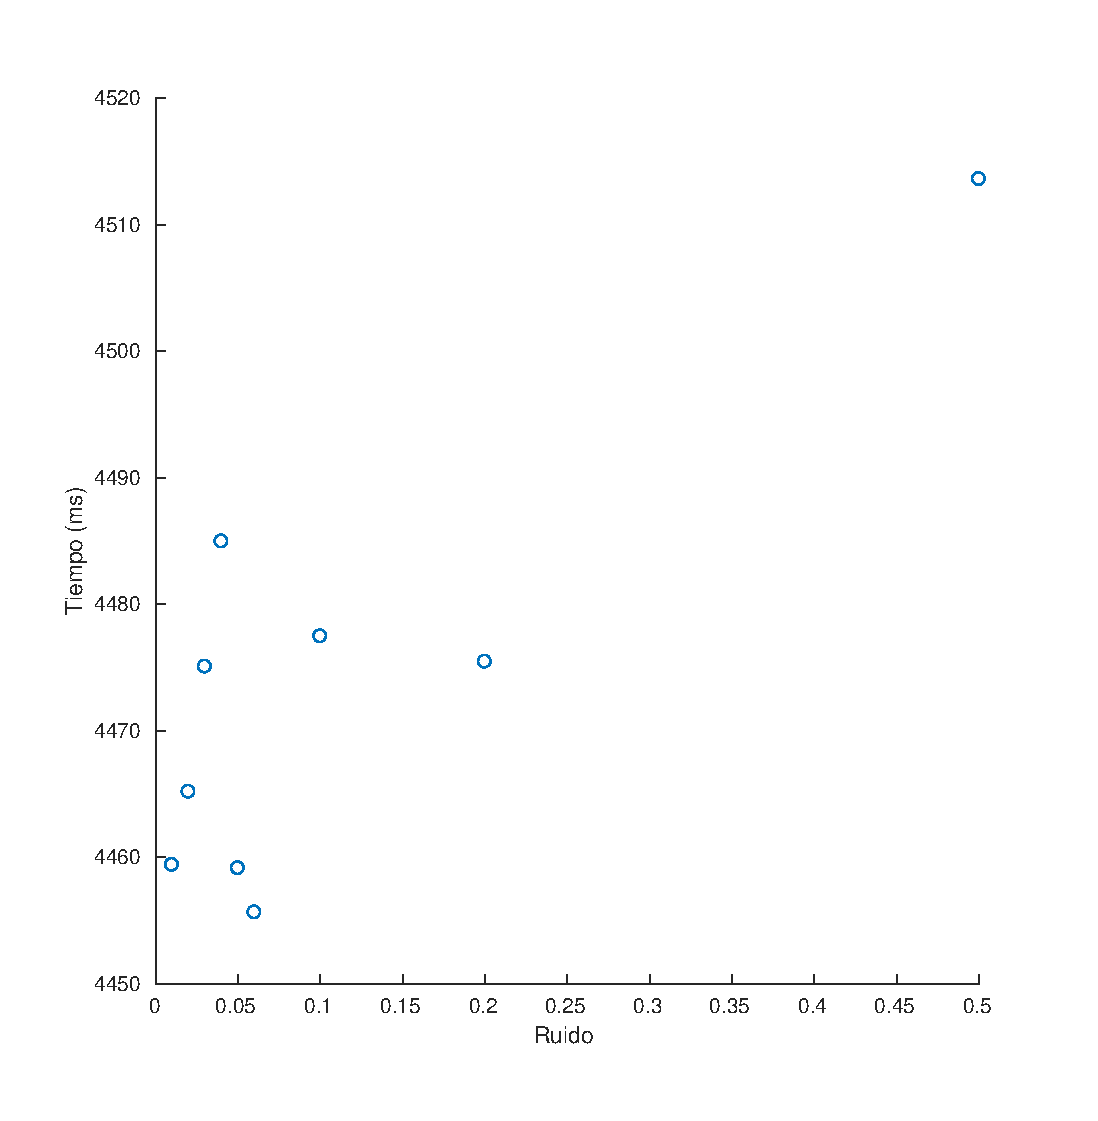
\includegraphics[width=0.7\textwidth]{img/ruido_tiempo}
	\caption{Tiempo en funcion del ruido con cantidad de rayos, cantidad de emisores y granularidad fijos}
	\label{fig:ruido_tiempo}
\end{figure}

\par Tal como esperabamos, el ruido que se le agrega a la imagen no afecta de manera significativa el tiempo de ejecuci\'on.

\begin{figure}[H]
	\centering	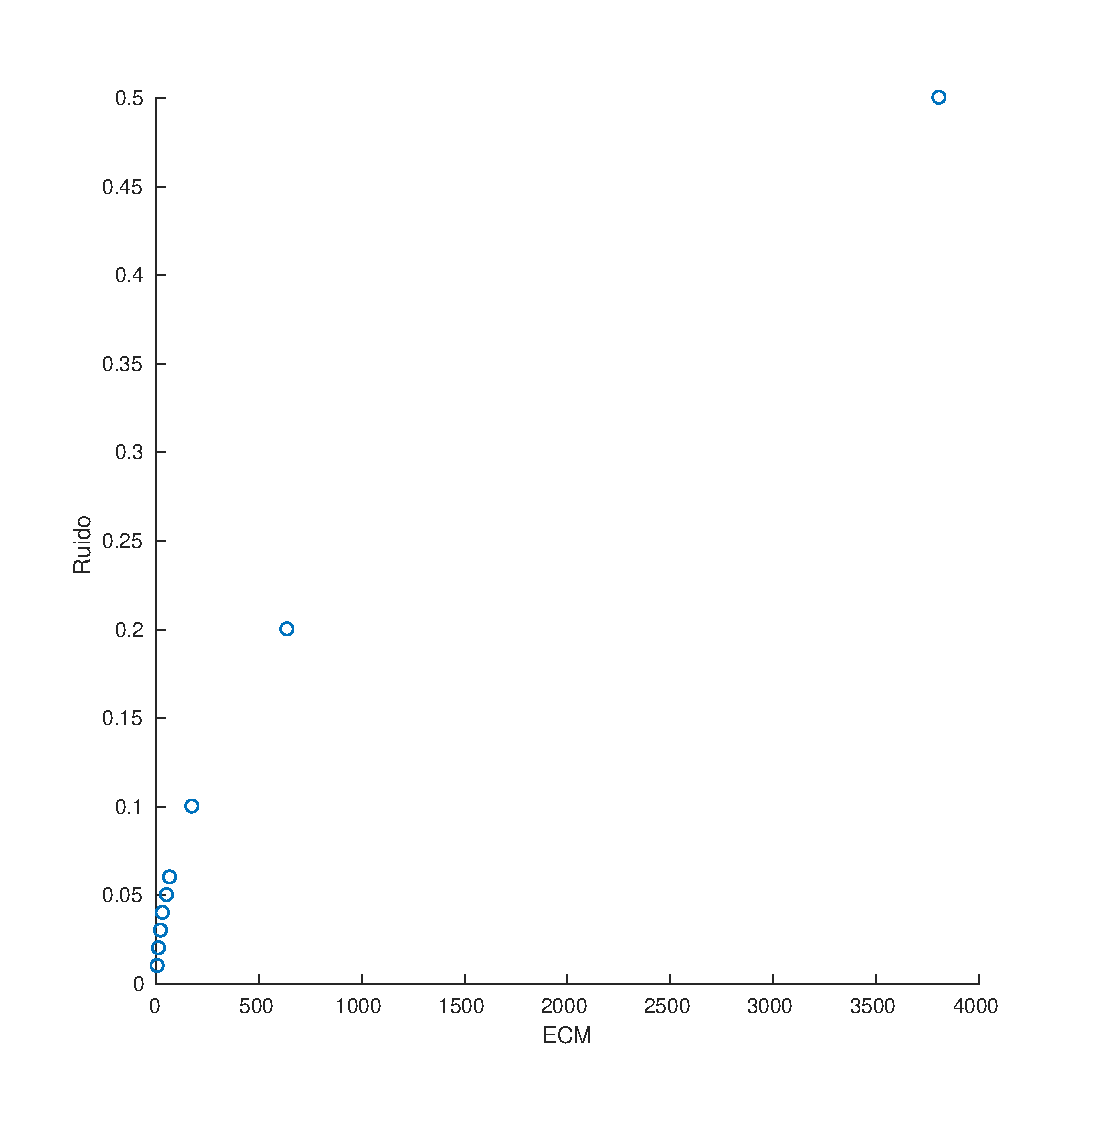
\includegraphics[width=0.7\textwidth]{img/ruido_ecm}
	\caption{ECM en funcion del ruido con cantidad de rayos, cantidad de emisores y granularidad fijos}
	\label{fig:ruido_ecm}
\end{figure}
\newpage


% \section{Discusión}
% Las expectativas que teníamos respecto de las pruebas usando solo KNN en comparación a KNN + PCA era que la segunda iba a dar mejores resultados en cuanto a las métricas de reconocimiento, sin embargo esto no fue así, lo que sí se logra usando PCA es trabajar con matrices más chicas, lo cual es útil si se trabaja con una base de datos con imágenes grandes o con muchas imágenes.
Con respecto a los tiempos tal como esperábamos PCA resulta lento en el procesamiento de la base de datos de entrenamiento sobre todo cuando se agregan muchas componentes principales. También suponíamos que las primeras componentes principales iban a influir más en tener buenos resultados de reconocimiento. Esto efectivamente fue así y lo usamos al diseñar los casos de test usando $\alpha$ más próximos en los valores pequeños y espaciándolos en valores más altos.
Una de las cosas que suponíamos es que usando un K más alto en KNN iba a funcionar mejor, pero esto no fue así, dando mejores métricas para K más chicos.
Los tiempos de ejecución fue una de las cuestiones que tuvimos en cuenta a a hora de diseñar los casos de pruebafundamentalmente en las corridas que usan PCA.
% \newpage

\section{Conclusiones}
\subsubsection*{Conclusiones}

\newpage

\section{Apendices}
\subsubsection*{Apendices}

\textbf{Parámetros de entrada:} Para correr el programa se deben utilizar los siguientes parámetros:
\begin{enumerate}
\item Nombre del archivo de entrada sin extensión. Se asume que el archivo es de tipo csv conteniendo imágenes de 16 bits.
\item Nivel de ruido: valor entre 0 y 1.
\item Dimension de la imagen: cantidad de pixeles por fila. Asumimos que la imagen es cuadrada.
\item Dimensión de celda. Número entero que debe s.er divisor de la cantidad de pixeles por fila de la imagen. Se asume que las celdas van a ser cuadradas.
\item Cantidad de Emisores. Cantidad total de emisores.
\item Cantidad de rayos. Cantidad de rayos que se van a trazar desde cada emisor.
\end{enumerate}
\par Ejemplo: $./tp3 ./imgs_TC/tomo 0.1 100 5 20 120$
\par Con estos parámetros se toma el archivo tomo.csv, nivel de ruido 0.1, dimension de la imagen 100x100 pixeles, dimensión de la celda 5x5 pixeles, 20 emisores, 120 rayos por emisor.

\par En el mismo directorio en que se encuentran las imágenes de entrada se genera el archivo que contiene la imagen reconstruida en format pgm de 8 bits. Tiene el mismo nombre que el archivo de entrada y extensión '.pgm'.

Analisis de las imágenes reconstruídas.

En el caso de las imágenes correspondientes a las pruebas que se realizaron variando la cantidad de emisores a simple vista se puede observar que los mejores resultados se dan con 60, 120 y 140 emisores mientras que valores intermedios producen resultados menos definidos. En el caso de los 60 emisores este resultado además es consistente con un menor valor del ECM pero en el caso de 120 y 140 emisores esa relación no es clara, incluso el error con 140 es más grande que con 80 emisores sin embargo la imagen resulta más nítida. Nos cuesta establecer una relación entre la cantidad de emisores y la definición de la imagen. Es posible que al elegir los ángulos de los rayos de forma aleatoria se pueda estar generando rayos muy parecidos que no aportan información relevante.

Algo similar ocurre con las pruebas hechas variando la cntidad de rayos, en las cuales podemos observar mejores resultados con una cantidad de 60 o de 100 rayos mientras que con 140 es practicamente irreconocible.

En el caso de las imágenes correspondientes a las pruebas que se realizaron variando la granularidad se puede ver que a una granularidad más fina se observan imágenes más definidas. Esto está además en correlación con los resultados obtenidos en el cálculo del ECM.



\begin{figure}[H]
    \centering	
\includegraphics[width=0.05\textwidth]{img/tomo_emisores_20.png}

\includegraphics[width=0.05\textwidth]{img/tomo_emisores_40.png}

\includegraphics[width=0.05\textwidth]{img/tomo_emisores_60.png}

\includegraphics[width=0.05\textwidth]{img/tomo_emisores_80.png}

\includegraphics[width=0.05\textwidth]{img/tomo_emisores_100.png}

\includegraphics[width=0.05\textwidth]{img/tomo_emisores_120.png}

\includegraphics[width=0.05\textwidth]{img/tomo_emisores_140.png}
	\caption{Reconstruccion de una imagen de 100x100 con 20, 40, 60, 80, 100, 120 y 140 emisores de rayos respectivamente}
	\label{fig:emisores}
\end{figure}


\begin{figure}[H]
    \centering	

\includegraphics[width=0.05\textwidth]{img/tomo_rayos_50.png}

\includegraphics[width=0.05\textwidth]{img/tomo_rayos_60.png}

\includegraphics[width=0.05\textwidth]{img/tomo_rayos_70.png}

\includegraphics[width=0.05\textwidth]{img/tomo_rayos_80.png}

\includegraphics[width=0.05\textwidth]{img/tomo_rayos_90.png}

\includegraphics[width=0.05\textwidth]{img/tomo_rayos_100.png}

\includegraphics[width=0.05\textwidth]{img/tomo_rayos_110.png}

\includegraphics[width=0.05\textwidth]{img/tomo_rayos_120.png}

\includegraphics[width=0.05\textwidth]{img/tomo_rayos_130.png}

\includegraphics[width=0.05\textwidth]{img/tomo_rayos_140.png}
	\caption{Reconstruccion de una imagen de 100x100 con 50, 60, 70, 80, 90, 100, 110, 120, 130 y 140 rayos por emisor respectivamente}
	\label{fig:rayos}
\end{figure}


\begin{figure}[H]
    \centering

\includegraphics[width=0.05\textwidth]{img/tomo_granu_5.png}

\includegraphics[width=0.05\textwidth]{img/tomo_granu_10.png}

\includegraphics[width=0.05\textwidth]{img/tomo_granu_20.png}

\includegraphics[width=0.05\textwidth]{img/tomo_granu_25.png}

\includegraphics[width=0.05\textwidth]{img/tomo_granu_50.png}
	\caption{Reconstruccion de una imagen de 100x100 con granularidad 5, 10, 15, 20 y 50 respectivamente}
	\label{fig:ruido}
\end{figure}


\begin{figure}[H]
    \centering

\includegraphics[width=0.05\textwidth]{img/tomo_ruido001.png}

\includegraphics[width=0.05\textwidth]{img/tomo_ruido002.png}

\includegraphics[width=0.05\textwidth]{img/tomo_ruido003.png}

\includegraphics[width=0.05\textwidth]{img/tomo_ruido004.png}

\includegraphics[width=0.05\textwidth]{img/tomo_ruido005.png}

\includegraphics[width=0.05\textwidth]{img/tomo_ruido006.png}

\includegraphics[width=0.05\textwidth]{img/tomo_ruido01.png}

\includegraphics[width=0.05\textwidth]{img/tomo_ruido05.png}
	\caption{Reconstruccion de una imagen de 100x100 con ruido 0.01, 0.02, 0.03, 0.04, 0.05, 0.06, 0.1, 0.5 respectivamente}
	\label{fig:emisores}
\end{figure}	
\newpage

\section{Referencias}
\subsubsection*{Referencias}
https://es.slideshare.net/sriAnkush/comparative-study-of-salt-pepper-filters-and-gaussian-filters

	
\newpage


\end{document}

